% !TEX TS-program = pdflatex
% !TEX encoding = UTF-8 Unicode

% This is a simple template for a LaTeX document using the "article" class.
% See "book", "report", "letter" for other types of document.

\documentclass[11pt]{article} % use larger type; default would be 10pt

\usepackage[utf8]{inputenc} % set input encoding (not needed with XeLaTeX)
\usepackage{tikz}
%%% Examples of Article customizations
% These packages are optional, depending whether you want the features they provide.
% See the LaTeX Companion or other references for full information.

%%% PAGE DIMENSIONS
\usepackage{geometry} % to change the page dimensions
\geometry{a4paper} % or letterpaper (US) or a5paper or....
% \geometry{margins=2in} % for example, change the margins to 2 inches all round
% \geometry{landscape} % set up the page for landscape
%   read geometry.pdf for detailed page layout information

\usepackage{graphicx} % support the \includegraphics command and options

% \usepackage[parfill]{parskip} % Activate to begin paragraphs with an empty line rather than an indent

%%% PACKAGES
\usepackage{booktabs} % for much better looking tables
\usepackage{array} % for better arrays (eg matrices) in maths
\usepackage{paralist} % very flexible & customisable lists (eg. enumerate/itemize, etc.)
\usepackage{verbatim} % adds environment for commenting out blocks of text & for better verbatim
\usepackage{subfig} % make it possible to include more than one captioned figure/table in a single float
% These packages are all incorporated in the memoir class to one degree or another...
\usepackage{url}
\usepackage{hyperref}

%%% HEADERS & FOOTERS
\usepackage{fancyhdr} % This should be set AFTER setting up the page geometry
\pagestyle{fancy} % options: empty , plain , fancy
\renewcommand{\headrulewidth}{0pt} % customise the layout...
\lhead{}\chead{}\rhead{}
\lfoot{}\cfoot{\thepage}\rfoot{}

%%% SECTION TITLE APPEARANCE
\usepackage{sectsty}
\allsectionsfont{\sffamily\mdseries\upshape} % (See the fntguide.pdf for font help)
% (This matches ConTeXt defaults)

%%% ToC (table of contents) APPEARANCE
\usepackage[nottoc,notlof,notlot]{tocbibind} % Put the bibliography in the ToC
\usepackage[titles,subfigure]{tocloft} % Alter the style of the Table of Contents
\renewcommand{\cftsecfont}{\rmfamily\mdseries\upshape}
\renewcommand{\cftsecpagefont}{\rmfamily\mdseries\upshape} % No bold!

%%% END Article customizations

%%% The "real" document content comes below...

\usepackage{amsfonts}
\usepackage{amsmath}
\usepackage{amsthm}

\theoremstyle{definition}
\newtheorem*{beispiel}{Beispiel}
\newtheorem{definition}{Definition}
\newtheorem*{bemerkung}{Bemerkung}
\newtheorem*{beweis}{Beweis}
\newtheorem*{ubung}{Übung}

\title{Theoretische Informatik -- Schreibomat}
\author{Florian}
%\date{} % Activate to display a given date or no date (if empty),
         % otherwise the current date is printed 

\begin{document}
\maketitle

\section*{Tools}
\begin{itemize}
\item Finite State Machine Designer: \url{http://madebyevan.com/fsm/}
\end{itemize}

\section{Was ist Informatik?}

\begin{itemize}

\item Konkrete\footnote{4. September 2012} Konzepte: Algorithmus, Berechnung, Komplexität

\item Was will die theoretische Informatik? Formale Bestimmung der Begriffe, unabhängig von Hard- und Software

\item Ziel: Grundlegende Eigenschaften von Algorithmen, Berechnungen erkennen. Methoden entwickeln zum Entwurf beweisbar korrekter Hard- und Software (nicht Schwerpunkt dieser Vorlesung)

\item Grenzen der automatischen Berechnung aufzeigen

\item Typische Fragestellungen: Ist es möglich, ein Programm zu schreiben, das ein anderes Programm als Eingabe erhält und feststellen kann, ob dieses in eine Endlosschleife gerät oder nicht? $\Rightarrow$ Halteproblem. Nein, es ist natürlich nicht möglich. Eine andere typische Fragestellung ist die Folgende: Wir haben einen Rucksack, und der hat 30 Liter Fassungsvermögen. Und wir haben noch 50 Gegenstände, und jetzt wollen wir wissen: wie lange dauert es, herauszufinden, wieviele Gegenstände in den Rucksack passen? Rucksackproblem, nicht in polynomialer Zeit lösbar $\Rightarrow$ Es dauert expontiell lange.

\item Leider ist es in der Praxis so, dass die Antwort auf ähnliche Fragestellungen nicht immer so offensichtlich ist, und deshalt müssen wir es uns ein bisschen genauer betrachten.

\end{itemize}

\begin{ubung}

Gegeben sei das folgende Strassennetz:

(Wildes Gekritzel)

\begin{enumerate}[(a)]
\item Gibt es eine Möglichkeit, alle Strassen genau 1x zu durchlaufen und dann wieder am Ausgangspunkt anzulangen,
\item Gibt es eine Möglichkeit, alle Kreuzungen genau 1x zu passieren und dann wieder am Ausgangspunkt anzulangen?
\end{enumerate}

Die Antworten sind imfall:
\begin{enumerate}[(a)]
\item Einfache Aufgabe: Geht immer, wenn die Anzahl der Abzweigungen an jeder Kreuzung gerade ist.
\item Traveling salesman (TSP). Schwierig! Es ist keine wesentlich bessere Methode bekannt, als einfach alles durchzuprobieren.
\end{enumerate}

\end{ubung}

Ziel für die Vorlesung: Um solche Fragestellungen systematisch beantworten zu können, brauchen wir ein exaktes mathematisches Modell eines Computers.

\section{Automatentheorie}

Endliche Automaten, Kontextfreie Grammatiken und Keller-Automaten. Zusätzliche Motivation: Das sind Konzepte, denen man auch häufig in der Praxis begegnet (Compilerbau, Textsuche, Textverarbeitung)

Noch nicht ganz so formal, bisschen intuitiv. Modellierung eines Kippschalters.

\begin{center}
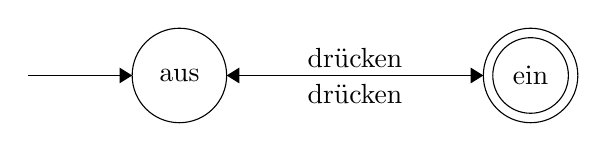
\begin{tikzpicture}[scale=0.2]
\tikzstyle{every node}+=[inner sep=0pt]
\draw [black] (23.8,-28.8) circle (3);
\draw (23.8,-28.8) node {aus};
\draw [black] (46.1,-28.8) circle (3);
\draw (46.1,-28.8) node {ein};
\draw [black] (46.1,-28.8) circle (2.4);
\draw [black] (26.8,-28.8) -- (43.1,-28.8);
\fill [black] (43.1,-28.8) -- (42.3,-28.3) -- (42.3,-29.3);
\draw (34.95,-29.3) node [below] {drücken};
\draw [black] (43.1,-28.8) -- (26.8,-28.8);
\fill [black] (26.8,-28.8) -- (27.6,-29.3) -- (27.6,-28.3);
\draw (34.95,-28.3) node [above] {drücken};
\draw [black] (14.2,-28.8) -- (20.8,-28.8);
\fill [black] (20.8,-28.8) -- (20,-28.3) -- (20,-29.3);
\end{tikzpicture}
\end{center}

\begin{definition}[Endlicher Automat]
Wir haben: \begin{itemize}
\item Zwei Zustände, davon ein Startzustand
\item und ein akzeptierender Zustand
\item Transitionen (Zustandsübergänge): führen den Automaten anhand einer Eingabe von einem Zusand in den nächsten.
\end{itemize}
\end{definition}

Beispiel: Mustererkennung in Texten: z.B. Suche das Wort "then"

\begin{center}
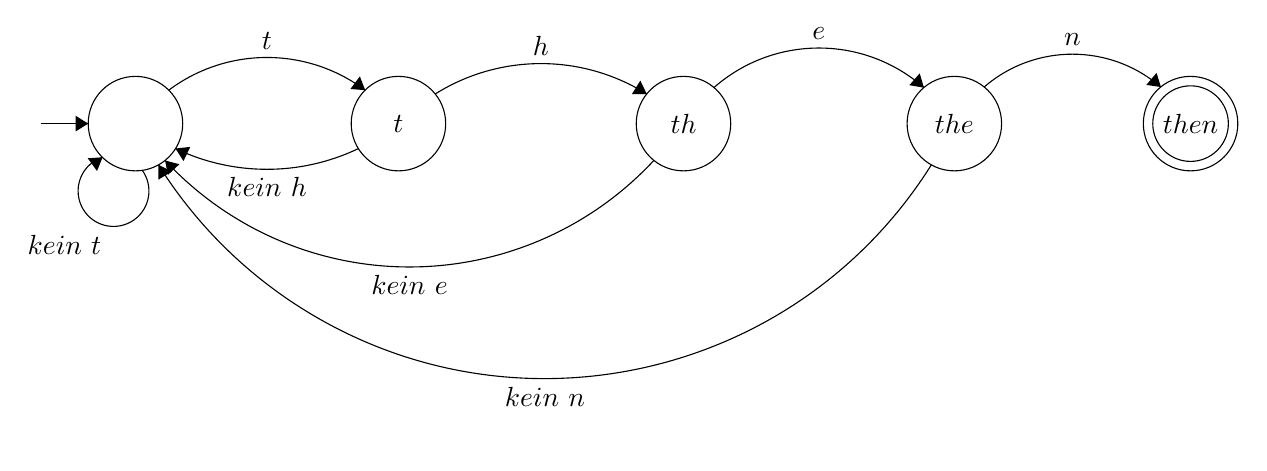
\begin{tikzpicture}[scale=0.2]
\tikzstyle{every node}+=[inner sep=0pt]
\draw [black] (7.4,-27.9) circle (3);
\draw [black] (24.1,-27.9) circle (3);
\draw (24.1,-27.9) node {$t$};
\draw [black] (42.2,-27.9) circle (3);
\draw (42.2,-27.9) node {$th$};
\draw [black] (59.4,-27.9) circle (3);
\draw (59.4,-27.9) node {$the$};
\draw [black] (74.4,-27.9) circle (3);
\draw (74.4,-27.9) node {$then$};
\draw [black] (74.4,-27.9) circle (2.4);
\draw [black] (1.4,-27.9) -- (4.4,-27.9);
\fill [black] (4.4,-27.9) -- (3.6,-27.4) -- (3.6,-28.4);
\draw [black] (9.509,-25.781) arc (126.87812:53.12188:10.4);
\fill [black] (21.99,-25.78) -- (21.65,-24.9) -- (21.05,-25.7);
\draw (15.75,-23.2) node [above] {$t$};
\draw [black] (26.43,-26.021) arc (122.09355:57.90645:12.649);
\fill [black] (39.87,-26.02) -- (39.46,-25.17) -- (38.93,-26.02);
\draw (33.15,-23.59) node [above] {$h$};
\draw [black] (44.128,-25.616) arc (131.3237:48.6763:10.104);
\fill [black] (57.47,-25.62) -- (57.2,-24.71) -- (56.54,-25.46);
\draw (50.8,-22.6) node [above] {$e$};
\draw [black] (61.283,-25.584) arc (130.87735:49.12265:8.583);
\fill [black] (72.52,-25.58) -- (72.24,-24.68) -- (71.59,-25.44);
\draw (66.9,-22.99) node [above] {$n$};
\draw [black] (7.827,-30.858) arc (35.95699:-252.04301:2.25);
\draw (2.89,-34.93) node [below] {$kein\mbox{ }t$};
\fill [black] (5.31,-30.04) -- (4.37,-30.1) -- (4.96,-30.91);
\draw [black] (21.56,-29.484) arc (-64.4345:-115.5655:13.463);
\fill [black] (9.94,-29.48) -- (10.45,-30.28) -- (10.88,-29.38);
\draw (15.75,-31.3) node [below] {$kein\mbox{ }h$};
\draw [black] (40.321,-30.235) arc (-42.87511:-137.12489:21.179);
\fill [black] (9.28,-30.24) -- (9.46,-31.16) -- (10.19,-30.48);
\draw (24.8,-37.5) node [below] {$kein\mbox{ }e$};
\draw [black] (57.939,-30.519) arc (-32.11581:-147.88419:28.973);
\fill [black] (8.86,-30.52) -- (8.86,-31.46) -- (9.71,-30.93);
\draw (33.4,-44.59) node [below] {$kein\mbox{ }n$};
\end{tikzpicture}
\end{center}

Getränkeautomat (Beispiel für Automat mit Ausgabe): Cola für CHF 2, Wasser für CHF 1. Münzannahme: Münzen zu 1, 2 CHF.

\begin{center}
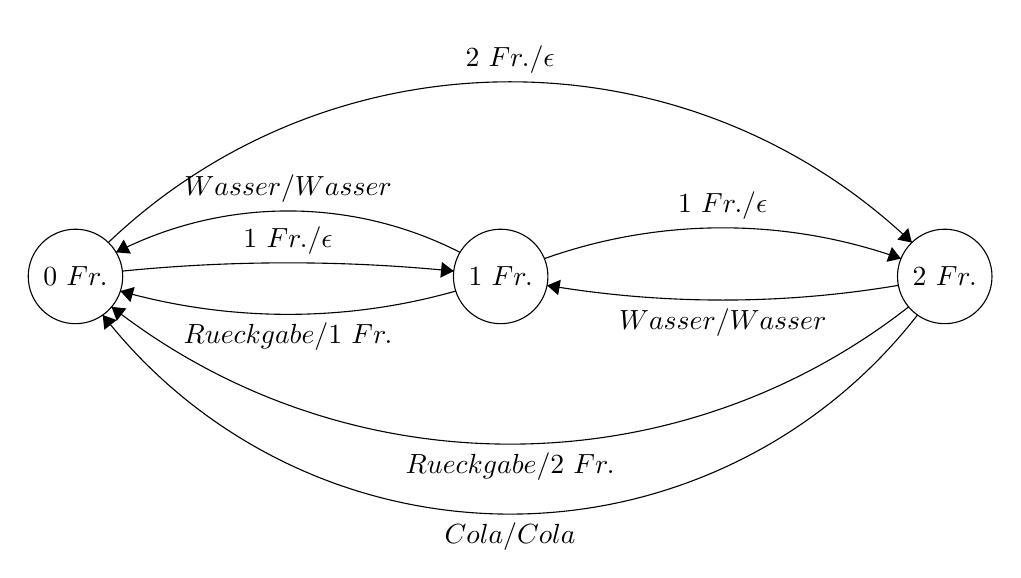
\begin{tikzpicture}[scale=0.2]
\tikzstyle{every node}+=[inner sep=0pt]
\draw [black] (8.2,-27.2) circle (3);
\draw (8.2,-27.2) node {$0\mbox{ }Fr.$};
\draw [black] (35.2,-27.2) circle (3);
\draw (35.2,-27.2) node {$1\mbox{ }Fr.$};
\draw [black] (63.4,-27.2) circle (3);
\draw (63.4,-27.2) node {$2\mbox{ }Fr.$};
\draw [black] (11.181,-26.859) arc (95.70544:84.29456:105.815);
\fill [black] (32.22,-26.86) -- (31.47,-26.28) -- (31.37,-27.28);
\draw (21.7,-25.84) node [above] {$1\mbox{ }Fr./\epsilon$};
\draw [black] (37.977,-26.069) arc (109.61489:70.38511:33.729);
\fill [black] (60.62,-26.07) -- (60.04,-25.33) -- (59.7,-26.27);
\draw (49.3,-23.61) node [above] {$1\mbox{ }Fr./\epsilon$};
\draw [black] (10.286,-25.045) arc (133.60946:46.39054:36.991);
\fill [black] (61.31,-25.05) -- (61.08,-24.13) -- (60.39,-24.86);
\draw (35.8,-14.34) node [above] {$2\mbox{ }Fr./\epsilon$};
\draw [black] (32.348,-28.128) arc (-74.17617:-105.82383:39.049);
\fill [black] (11.05,-28.13) -- (11.69,-28.83) -- (11.96,-27.87);
\draw (21.7,-30.11) node [below] {$Rueckgabe/1\mbox{ }Fr.$};
\draw [black] (61.106,-29.132) arc (-51.98339:-128.01661:41.089);
\fill [black] (10.49,-29.13) -- (10.82,-30.02) -- (11.43,-29.23);
\draw (35.8,-38.35) node [below] {$Rueckgabe/2\mbox{ }Fr.$};
\draw [black] (10.779,-25.671) arc (117.08879:62.91121:23.983);
\fill [black] (10.78,-25.67) -- (11.72,-25.75) -- (11.26,-24.86);
\draw (21.7,-22.54) node [above] {$Wasser/Wasser$};
\draw [black] (61.668,-29.648) arc (-37.90364:-142.09636:32.784);
\fill [black] (9.93,-29.65) -- (10.03,-30.59) -- (10.82,-29.97);
\draw (35.8,-42.79) node [below] {$Cola/Cola$};
\draw [black] (60.454,-27.765) arc (-80.41933:-99.58067:67.017);
\fill [black] (38.15,-27.77) -- (38.85,-28.39) -- (39.02,-27.41);
\draw (49.3,-29.2) node [below] {$Wasser/Wasser$};
\end{tikzpicture}
\end{center}

Wenn der Automat nur eine Flasche Cola und eine Flasche Wasser enthält:

\begin{center}
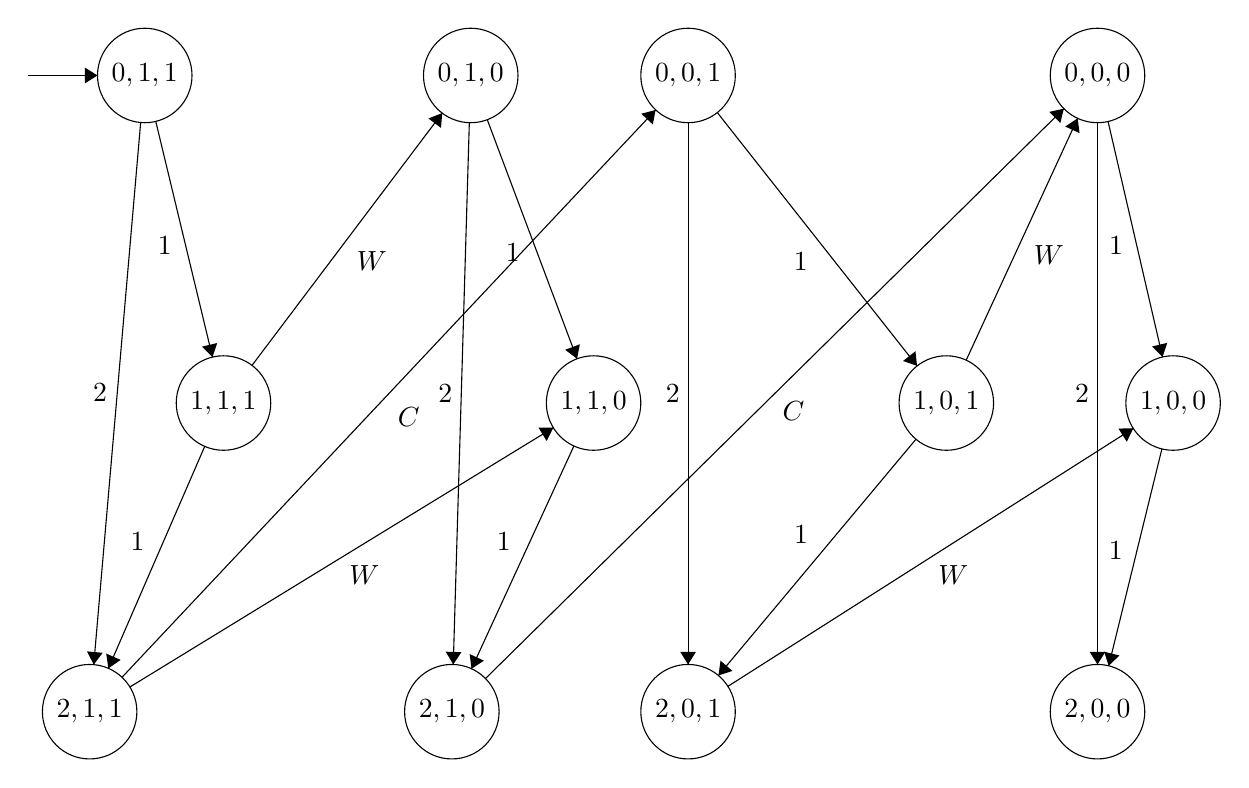
\begin{tikzpicture}[scale=0.2]
\tikzstyle{every node}+=[inner sep=0pt]
\draw [black] (9.8,-7.7) circle (3);
\draw (9.8,-7.7) node {$0,1,1$};
\draw [black] (30.5,-7.7) circle (3);
\draw (30.5,-7.7) node {$0,1,0$};
\draw [black] (44.3,-7.7) circle (3);
\draw (44.3,-7.7) node {$0,0,1$};
\draw [black] (14.8,-28.5) circle (3);
\draw (14.8,-28.5) node {$1,1,1$};
\draw [black] (38.3,-28.5) circle (3);
\draw (38.3,-28.5) node {$1,1,0$};
\draw [black] (60.7,-28.5) circle (3);
\draw (60.7,-28.5) node {$1,0,1$};
\draw [black] (70.3,-7.7) circle (3);
\draw (70.3,-7.7) node {$0,0,0$};
\draw [black] (75.1,-28.5) circle (3);
\draw (75.1,-28.5) node {$1,0,0$};
\draw [black] (6.3,-48.1) circle (3);
\draw (6.3,-48.1) node {$2,1,1$};
\draw [black] (29.3,-48.1) circle (3);
\draw (29.3,-48.1) node {$2,1,0$};
\draw [black] (44.3,-48.1) circle (3);
\draw (44.3,-48.1) node {$2,0,1$};
\draw [black] (70.3,-48.1) circle (3);
\draw (70.3,-48.1) node {$2,0,0$};
\draw [black] (2.4,-7.7) -- (6.8,-7.7);
\fill [black] (6.8,-7.7) -- (6,-7.2) -- (6,-8.2);
\draw [black] (10.5,-10.62) -- (14.1,-25.58);
\fill [black] (14.1,-25.58) -- (14.4,-24.69) -- (13.43,-24.92);
\draw (11.54,-18.53) node [left] {$1$};
\draw [black] (9.54,-10.69) -- (6.56,-45.11);
\fill [black] (6.56,-45.11) -- (7.13,-44.36) -- (6.13,-44.27);
\draw (7.43,-27.83) node [left] {$2$};
\draw [black] (31.55,-10.51) -- (37.25,-25.69);
\fill [black] (37.25,-25.69) -- (37.43,-24.77) -- (36.5,-25.12);
\draw (33.64,-18.92) node [left] {$1$};
\draw [black] (30.41,-10.7) -- (29.39,-45.1);
\fill [black] (29.39,-45.1) -- (29.91,-44.32) -- (28.91,-44.29);
\draw (29.36,-27.89) node [left] {$2$};
\draw [black] (44.3,-10.7) -- (44.3,-45.1);
\fill [black] (44.3,-45.1) -- (44.8,-44.3) -- (43.8,-44.3);
\draw (43.8,-27.9) node [left] {$2$};
\draw [black] (46.16,-10.06) -- (58.84,-26.14);
\fill [black] (58.84,-26.14) -- (58.74,-25.21) -- (57.95,-25.83);
\draw (51.93,-19.52) node [left] {$1$};
\draw [black] (70.3,-10.7) -- (70.3,-45.1);
\fill [black] (70.3,-45.1) -- (70.8,-44.3) -- (69.8,-44.3);
\draw (69.8,-27.9) node [left] {$2$};
\draw [black] (70.97,-10.62) -- (74.43,-25.58);
\fill [black] (74.43,-25.58) -- (74.73,-24.68) -- (73.76,-24.91);
\draw (71.95,-18.5) node [left] {$1$};
\draw [black] (13.61,-31.25) -- (7.49,-45.35);
\fill [black] (7.49,-45.35) -- (8.27,-44.81) -- (7.35,-44.41);
\draw (9.82,-37.33) node [left] {$1$};
\draw [black] (37.05,-31.23) -- (30.55,-45.37);
\fill [black] (30.55,-45.37) -- (31.34,-44.86) -- (30.43,-44.44);
\draw (33.08,-37.28) node [left] {$1$};
\draw [black] (58.77,-30.8) -- (46.23,-45.8);
\fill [black] (46.23,-45.8) -- (47.12,-45.51) -- (46.36,-44.86);
\draw (51.95,-36.86) node [left] {$1$};
\draw [black] (74.39,-31.41) -- (71.01,-45.19);
\fill [black] (71.01,-45.19) -- (71.69,-44.53) -- (70.72,-44.29);
\draw (71.94,-37.86) node [left] {$1$};
\draw [black] (16.61,-26.11) -- (28.69,-10.09);
\fill [black] (28.69,-10.09) -- (27.81,-10.43) -- (28.61,-11.03);
\draw (23.23,-19.5) node [right] {$W$};
\draw [black] (8.86,-46.53) -- (35.74,-30.07);
\fill [black] (35.74,-30.07) -- (34.8,-30.06) -- (35.32,-30.91);
\draw (23.74,-38.8) node [below] {$W$};
\draw [black] (8.36,-45.91) -- (42.24,-9.89);
\fill [black] (42.24,-9.89) -- (41.33,-10.13) -- (42.06,-10.81);
\draw (25.83,-29.37) node [right] {$C$};
\draw [black] (31.44,-45.99) -- (68.16,-9.81);
\fill [black] (68.16,-9.81) -- (67.24,-10.01) -- (67.94,-10.72);
\draw (50.99,-28.38) node [below] {$C$};
\draw [black] (61.96,-25.78) -- (69.04,-10.42);
\fill [black] (69.04,-10.42) -- (68.25,-10.94) -- (69.16,-11.36);
\draw (66.22,-19.13) node [right] {$W$};
\draw [black] (46.83,-46.49) -- (72.57,-30.11);
\fill [black] (72.57,-30.11) -- (71.63,-30.12) -- (72.16,-30.96);
\draw (61.14,-38.8) node [below] {$W$};
\end{tikzpicture}
\end{center}

\section{Formale Sprachen}

Ziel: Genaue Beschreibung der Ein- und Ausgaben eines Automaten.

\begin{definition}[Alphabet]
(endliche, nichtleere Menge von Symbolen). Bsp: Binäres Alphabet $\Sigma_{\textrm{bin}} = \{0,1\}$, Tastaturalphabet $\Sigma_{\textrm{tast}} = \{ a, \dots, z, A, \dots, Z, 0, \dots 9, \dots \}$
\end{definition}

\begin{definition}[Wort (= Zeichenkette, String)]
Endliche Folge von Symbolen eines gegebenen Alphabets. Beispiel: 01110 ist ein Wort über $\Sigma_{\textrm{bin}}$.
\end{definition}

\begin{bemerkung}[Eigenschaften von Wörtern]
Die da wären:
\begin{itemize}
\item Leeres Wort: $\epsilon$ (manchmal $\lambda$) = leere Folge von Symbolen (über einem beliebigen Alphabet)
\item Länge eines Wortes: $|w|$ bezeichnet die Anzahl der Symbole im Wort $w$. $|\epsilon| = 0$.
\end{itemize}
\end{bemerkung}

\begin{bemerkung}[Konventionen für Darstellung von Wörtern]
Wir sagen:
\begin{itemize}
\item $a,b,c,\dots$ für Buchstaben, Symbole
\item $v,w,x,\dots$ für Wörter
\end{itemize}
\end{bemerkung}

\begin{definition}[Potenzen von Wörtern]
Es gibt im Angebot:
\begin{itemize}
\item Menge aller Wörter einer bestimmten Länge:
\begin{eqnarray*}
\textrm{Sei $\Sigma$ Alphabet, so:} && \\
 \Sigma^0 &=& \{\epsilon\} \\
 \Sigma^1 &=& \Sigma \\
\Sigma^2 &=& \{ ab | a,b \in \Sigma\} \\
\Sigma^i &=& \{ a_1\dots a_i | a_1 \dots a_i \in \Sigma \}
\end{eqnarray*}
\item Menge aller Wörter über $\Sigma$: \[
\Sigma^* = \bigcup\limits_{i = 0}^{\infty} \Sigma^i, \epsilon \in \Sigma^*
\]
\item Menge aller nichtleeren Wörter über $\Sigma$: \[
\Sigma^+ = \bigcup\limits_{i = 1}^{\infty} \Sigma^i, \epsilon \notin \Sigma^+
\]
\end{itemize}
\end{definition}
\begin{beispiel}
\item Beispiel: \begin{eqnarray*}
\Sigma &=& \{0,1\} \\
\Sigma^2 &=& \{00, 01, 10, 11\} \\
\Sigma^* &=& \{\epsilon, 0, 1, 00, 01, 10, 11, 000, 001, \dots \}
\end{eqnarray*}
\end{beispiel}

\begin{definition}[Konkatenation (Verkettung) von Wörtern]
\[
v = a_1,\dots a_k, w = b_1\dots,b_k \textrm{ über } \Sigma \Rightarrow v\cdot w = a_1\dots a_kb_1\dots b_k = vw
\]
\end{definition}

\begin{bemerkung}[Rechenregeln für Konkatenation von Wörtern]
\begin{eqnarray*}
v\cdot(v\cdot w) &=& (u\cdot v)\cdot w \\
|x\cdot y| &=& |x| + |y| \\
x\cdot\epsilon&=&\epsilon\cdot x =  x
\end{eqnarray*}
\end{bemerkung}

\begin{bemerkung}[Infixe, Präfixe, Suffixe]
Seien $v,w \in \Sigma^*$ für ein Alphabet $\Sigma$, dann ist $v$ ein Teilwort (Infix) von $w$, falls es $x,y \in \Sigma^*$ gibt, so dass $w = x\cdot v \cdot y$; $v$ ist ein Präfix von $w$, falls es $y \in \Sigma^*$ gibt, so dass $w = v\cdot y$. Suffix funktionert analog.

Beispiel: abc ist Teilwort von aabcc, aa ist Präfix und Suffix von aabcaa. $\epsilon$ ist Teilwort von jedem Wort.
\end{bemerkung}

\begin{definition}[Sprache]
$L$ über Alphabet $\Sigma$ ist eine Teilmenge von $\Sigma^*$, $L \subseteq \Sigma^*$. Sprache ist Menge von Wörtern, kann unendlich gross sein. Leere Sprache: $\emptyset$ enthält keine Wörter, ist über jedem Alphabet definiert. Spezielle Sprache: $L_\epsilon$ ist die Sprache, die nur das leeere Wort enthält. $L_\epsilon \neq \emptyset$.
\end{definition}

\begin{definition}[Konkatenation von Sprachen] 
$L_1, L_2 \subseteq \Sigma^* \Rightarrow L_1 \cdot L_2 = L_1L_2 = \{ v\cdot w | v\in L_1, w\in L_2 \}$
\end{definition}
\begin{definition}[Potenzen von Sprachen]
\begin{eqnarray*}
L^0 &=& L_\epsilon = \{\epsilon\} \\
L^{i+1} &=& L^i\cdot L \textrm{ für } i \in \mathbb{N}
\end{eqnarray*}
\end{definition}

\begin{definition}[Kleene-Stern] 
\begin{eqnarray*}
L^* &=& \bigcup\limits_{i\in \mathbb{N}}^{} L^i \\
L^+ &=& \bigcup\limits_{i\in \mathbb{N}}^{} L^i - L_\epsilon
\end{eqnarray*}
\end{definition}

\begin{beispiel}
Sei $\Sigma = \{a,b\}, L_1 = \{a^i | i \ge 0\} = \{\epsilon, a, aa, aaa, \dots\}, L_2 = \{b^i | i \ge 0\} = \{\epsilon, b, bb, bbb, \dots\}$:

$L_1\cdot L_2 = \{ \epsilon, a,b,ab,aab,abb,aaab,\dots \} = \{a^ib^j | i \ge 0, j \ge 0 \}$ ist die Menge aller Wörter über $\{a,b\}$, in dem alle $a$s vor allen $b$s vorkommen.
\end{beispiel}

\begin{ubung}
Seien $L_1, L_2, L_3 \subseteq \Sigma^*$. 

(a) Gilt $(L_1\cdot L_2)\cdot L_3 =L_1\cdot(L_2\cdot L_3 )$? Ja.

(b) Gilt $(L_1\cup L_2)\cdot L_3 = L_1\cdot L_3 \cup L_2 \cdot L_3$? Ja.

(c) Gilt $(L_1\cdot L_2)\cup L_3 = (L_1\cup L_3) \cdot (L_2\cup L_3)$? Quatsch.

(d) Gilt $L_1\cdot L_2 = L_2\cdot L_1$? Quatsch.

\end{ubung}

\begin{proof}[Beweis]
(a)
\begin{eqnarray*}
(L_1\cdot L_2) \cdot L_3 &=& \{ vw | v \in L_1\cdot L_2, w \in L_3 \} \\
&=&\{xyw | x\in L_1, y \in L_2, w \in L_3 \} \\
&=& \{xz | x \in L_1, z \in L_2 L_3 \} \\
&=& L_1\cdot (L_2\cdot L_3)
\end{eqnarray*}

(b)
\begin{eqnarray*}
(L_1 \cup L_2) \cdot L_3 &=& \{vw | v \in L_1 \cup L_2, w \in L_3 \} \\
&=& \{vw | v \in L_1, w \in L_3 \} \cup \{ vw | v \in L_2, w \in L_3 \} \\
&=& (L_1\cdot L_3) \cup (L_2 \cdot L_3)
\end{eqnarray*}

(c)
Gegenbeispiel: $L_1 = L_2 = \{a\}, L_3 = \{b \}$. Daraus folgt:
\begin{eqnarray*}
L_1 L_2 = \{aa\} &\Rightarrow& (L_1 L_2)\cup L_3 = \{aa,b \} \\
L_1 \cup L_3 = \{a,b\} = L_2 \cup L_3 &=& \Rightarrow ...
\end{eqnarray*}

\end{proof}

\begin{bemerkung}
(d) gilt aber für $|\Sigma|$ = 1.
\end{bemerkung}

\begin{definition}[Entscheidungsproblem]
Die Eingabe ist eine Sprache $L$ über einem Alphabet $\Sigma$ sowie ein Wort $w \in \Sigma^*$. Die Ausgabe soll lauten: JA falls $w \in L$ oder NEIN falls $w \notin L$.

Die Modellierung von vielen alltäglichen Berechnungsproblemen im Formalismus der formalen Sprachen.
\end{definition}

\begin{beispiel}[Primzahltest]
Das Alphabet $\Sigma = \{0,1\}$. Die Sprache 
\[
L = \{w \in \Sigma^* | w \textrm{ ist Binärdarstellung einer Primzahl}  \}
\]

Eine Zahl $p \in N$ ist Primzahl genau dann, wenn $Bin(p) \in L$.

Identifizierung von Sprachen als Probleme.
\end{beispiel}

\section{Kurze Einführung in formale Beweise}

Behauptungen\footnote{11. September 2012} mit Unanfechtbarkeitsanspruch wollen bewiesen werden. Insbesondere negative Aussagen der Form "Dieses Rechenmodell kann diese Aufgabe nicht lösen" brauchen eine präzise Formulierung und Begründung, um glaubwürdig zu sein\footnote{Hopcraft et al., Abschnitt 1.2--1.4}\marginpar{Unkontrollierte Hausaufgabe}.

Als Beweismethoden haben wir im Angebot:

\begin{description}
\item[Deduktion (zum Beweis einer Implikation)] Zum Beweis von Wenn-Dann-Aussagen, z.B.
\[
\textrm{Wenn } \underbrace{x \ge 4}_{\textrm{Hypothese}}\textrm{ , dann } \underbrace{x^2\ge 16}_{\textrm{Konklusion}}
\]

Vorgehen: Hypothese als wahr annehmen, dann Folgerungen darauf anwenden, bis die Konklusion folgt.

\begin{beispiel}
Sei $x \ge 4$. Es gilt $4^2 = 16$ und die Quadratfunktion ist steigend. Daraus folgt: $x^2 \ge 4^2 = 16$
\end{beispiel}

Hierfür ist es oft hilfreich, Definitionen von Begriffen einzusetzen.
\begin{beispiel}
Wenn $L = \{ w \in \{a,b\}^* | |w| \textrm{ gerade}\}$, dann gilt für alle $x \in L^2$, dass $|x|$ gerade ist.
\end{beispiel}

\begin{proof}[Beweis]
Sei $x \in L^2$.

Definition von $L^2$ einsetzen. Es existieren $u,v \in L$, so dass $x = uv$.

Definition von $L$ einsetzen. $|u|$ ist gerade, $|v|$ ist gerade.

$\Rightarrow |x| = |u| + |v| \Rightarrow |x|$ ist gerade.
\end{proof}

\item[Doppelte Deduktion (zum Beweis einer Äquivalenz)] Zerlegung in zwei Wenn-Dann-Aussagen, wird getrennt bewiesen.

\begin{beispiel}[Gleichheit von Mengen]
\[
A = B \Rightarrow A \subseteq B \land B \subseteq A \Rightarrow A = B
\]

\end{beispiel}

\begin{beispiel}
Sprachen sind ja auch Mengen. Also: seien $L_1, L_2 \in \Sigma^*$. Dann gilt:
\[
L_1\cdot(L_1 \cup L_2) = L_1^2 \cup L_1 \cdot L_2
\]
\end{beispiel}

\begin{proof}[Beweis]
\begin{itemize}
Zweimal:
\item "$\subseteq$":

Sei $x \in L_1\cdot(L_1\cup L_2) \Rightarrow \exists x = uv, u \in L_1, v \in L_1 \cup L_2$.

Fallunterscheidung: (a) $v \in L_1 \Rightarrow x = uv, u \in L_1, v \in L_1 \Rightarrow x \in L_1^2$.

(b) $v \in L_2 \Rightarrow x = uv, u \in L_1, v \in L_2 \Rightarrow x \in L_1\cdot L_2$.

\item "$\supseteq$":

Sei $x \in L_1^2 \cup L_1\cdot L_2$.

Fallunterscheidung: (a) $x \in L_1^2 \Rightarrow x = uv, u, v \in L_1 $

$\Rightarrow v \in L_1 \cup L_2$

$\Rightarrow x \in L_1\cdot(L_1 \cup L_2)$.

(b) $x \in L_1\cdot L_2 \Rightarrow x = uv, u \in L_1, v \in L_2$

$\Rightarrow v \in (L_1 \cup L_2)$

$\Rightarrow x \in L_1\cdot(L_1 \cup L_2)$
\end{itemize}
\end{proof}

\item[Widerspruchsbeweis] Es wird eine Annahme getroffen und dann solange gefolgert, bis Quatsch herauskommt. Daraus folgt, dass die Annahme auch falsch sein muss.

\begin{beispiel}
Seien $a,b \in \mathbb{N}$ und $a,b \ge 2$. Dann gilt: $a$ teilt nicht $ab + 1$.
\end{beispiel}
\begin{proof}[Beweis]
Seien $a,b \in \mathbb{N}$. Angenommen, $a$ teilt $ab + 1$.

Ziel: Annahme zum Widerspruch führen, dann folgt daraus Negation, also die gewünschte Konklusion.

$a$ teilt $ab \Rightarrow a$ teilt $ab$ und $ab + 1$.

$\Rightarrow a$ teilt $(ab + 1)-(ab) = 1$

$\Rightarrow a = 1$. Bonk! Widerspruch zu $a \ge 2$.
\end{proof}

\begin{beispiel}
Es gibt unendlich viele Primzahl (äquivalente Formulierung: Es gibt keine grösste Primzahl).
\end{beispiel}

\begin{proof}[Beweis]
Angenommen, es gäbe eine grösste Primzahl. Wir nennen die Anzahl der Primzahlen $k$.

Seien $p_1 < p_2 < \dots < p_k$ die Primzahlen. Betrachten wir $x = p_1\cdot p_2 \cdot \dots \cdot p_k + 1$. Da $p_k$ die grösste Primzahl ist und $x > p_k$, kann $x$ keine Primzahl sein.

Also gibt es eine Primfaktorzerlegung von $x$, und $p_l$ sei die kleinste Primzahl in dieser Zerlegung.

Dann gilt: $p_l$ teilt $p_1\cdot p_2 \cdot dots \cdot p_k$ und $p_l$ teilt darum auch $x$.

Daraus folgt: $p_l$ teilt  $p_1\cdot p_2 \cdot dots \cdot p_k+1$. Aus dem vorhergehenden Beweis ($a$ teilt $ab+1$) folgt, dass das ein Widerspruch ist.
\end{proof}

\item[Induktion] Vor allem verwendet für Beweise über natürliche Zahlen. Ziel: Zeige, dass die Aussage $S(n)$ für alle $n \ge n_0$ gilt.

Methode:
\begin{enumerate}
\item Induktionsanfang (Anker). Zeige $S(n_0)$.
\item Induktionsschritt. Zeige $S(i) \Rightarrow S(i+1)$.
\end{enumerate}

Idee: Wenn $S(n_0)$ gilt und $S(i) \Rightarrow S(i+1)$ für alle $i \ge n_0$, dann folgt aus $S(n_0)$ und $S(n_0) \Rightarrow S(n_0+1)$, dann gilt $S(n_0+1)$. Undsoweiter, undsofort.

\begin{beispiel}[Der kleine Gauss].
Für alle $n \ge 1$ gilt: $\sum\limits_{i=1}^n i = \frac {n(n+1)} 2$
\end{beispiel}
\begin{proof}[Beweis]
Anker: $\sum\limits_{i=1}^1 = \frac{1+(1+1)}2$

Schritt: es gelte $\sum\limits_{i=1}^k i = \frac{k(k+1)} 2$ (Induktionsvoraussetzung).

Zeige: $\sum\limits_{i=1}^{k+1} i = \frac{(k+1)(k+1+1)} 2$ (Induktionsbehauptung).

\begin{eqnarray*}
\sum\limits_{i=1}^{k+1} i &=& \sum\limits_{i=1}^{k} i + (k+1) \\
&=& \frac{k(k+1)} 2 + (k+1) \\
&=& \frac{k(k+1) + 2(k+1)}2 \\
&=& \frac{(k+2)(k+1)}2 \\
&=& \frac{(k+1+1)(k+1)}2
\end{eqnarray*}
\end{proof}

\item[Rekursive Definitionen und strukturelle Induktion]
\begin{beispiel}[Rekursive Definition von arithmetischen Ausdrücken]
Basis: Jede Zahl und jede Variable ist ein arithmetischer Ausdruck: $(a+3)\cdot 5$ ist ein arithmetischer Ausdruck, $(a +3\cdot 5$ [sic] ist keiner (Klammerfehler).

Rekursion: Wenn $E$ und $F$ Ausdrücke sind, dann definieren wir, dass dann auch $E+F$, $E\cdot F$, $(E)$ arithmetische Ausdrücke sind.

Behauptung: Jeder Ausdruck enthält gleichviele linke wie rechte Klammern.
\end{beispiel}

\begin{proof}[Beweis] Mit struktureller Induktion:

\begin{enumerate}
\item I.A.: Basisausdrücke haben keine Klammern. Daraus folgt: gleichviele linke wie rechte Klammern (0).
\item Sei $G$ ein arithmetischer Ausdruck ($G = E+F, E\cdot F, (G)$). Fallunterscheidung:
\begin{enumerate}
\item $G=E+F$: Induktionsvoraussetzung: $E$ und $F$ haben gleich viele linke wie rechte Klammern. Gilt also auch für $G$, da keine Klammern hinzukommen.
\item $G=E\cdot F$: analog.
\item $(G)$: Induktionsvoraussetzung: $E$ hat gleich viele linke wie rechte Klammern. Gilt also auch für $G$, da 1 linke und 1 rechte Klammer hinzukommt.
\end{enumerate}
\end{enumerate}
\end{proof}

\end{description}

\section{Unendlichkeit}

\begin{proof}[Beweis für 3.7]
Behauptung: $|A| < |B| \Leftarrow |A| = |C| \land C \subset B$

$A = B = \mathbb{N} = \{0,1,2,3,\dots\}$
$C = \{1,2,3,4,\dots\}$
$(0,1), (1,2), \dots, (k,k+1)$
\end{proof}

Aufgaben: 3.7, 3.8, 3.11, 3.17, 3.18, 3.19

\section{Endliche Automaten}

Unterscheidung:
\begin{description}
\item[Deterministisch] Automat kann zu einem Zeitpunkt nur einen Zustand annehmen.
\item[Nichtdeterministisch] Automat kann gleichzeitig mehrere Zustände besitzen.
\end{description}

\begin{beispiel}
DEA zum Erkennen des Musters aba:

\begin{center}
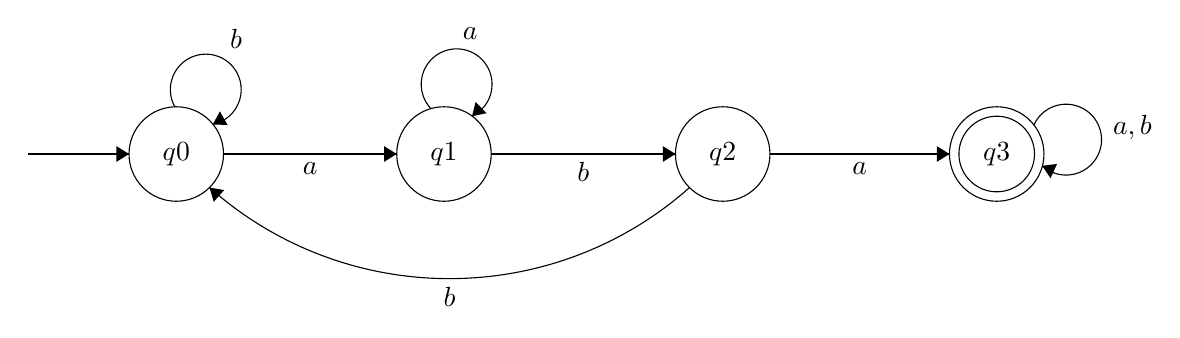
\begin{tikzpicture}[scale=0.2]
\tikzstyle{every node}+=[inner sep=0pt]
\draw [black] (15.3,-25.4) circle (3);
\draw (15.3,-25.4) node {$q0$};
\draw [black] (32.3,-25.4) circle (3);
\draw (32.3,-25.4) node {$q1$};
\draw [black] (50,-25.4) circle (3);
\draw (50,-25.4) node {$q2$};
\draw [black] (67.4,-25.4) circle (3);
\draw (67.4,-25.4) node {$q3$};
\draw [black] (67.4,-25.4) circle (2.4);
\draw [black] (5.9,-25.4) -- (12.3,-25.4);
\fill [black] (12.3,-25.4) -- (11.5,-24.9) -- (11.5,-25.9);
\draw [black] (18.3,-25.4) -- (29.3,-25.4);
\fill [black] (29.3,-25.4) -- (28.5,-24.9) -- (28.5,-25.9);
\draw (23.8,-25.9) node [below] {$a$};
\draw [black] (35.3,-25.4) -- (47,-25.4);
\fill [black] (47,-25.4) -- (46.2,-24.9) -- (46.2,-25.9);
\draw (41.15,-25.9) node [below] {$b$};
\draw [black] (53,-25.4) -- (64.4,-25.4);
\fill [black] (64.4,-25.4) -- (63.6,-24.9) -- (63.6,-25.9);
\draw (58.7,-25.9) node [below] {$a$};
\draw [black] (15.214,-22.413) arc (209.37644:-78.62356:2.25);
\draw (19.09,-18.76) node [above] {$b$};
\fill [black] (17.62,-23.52) -- (18.56,-23.56) -- (18.07,-22.69);
\draw [black] (31.478,-22.527) arc (223.69515:-64.30485:2.25);
\draw (33.97,-18.17) node [above] {$a$};
\fill [black] (34.08,-23) -- (35,-22.81) -- (34.31,-22.09);
\draw [black] (47.892,-27.531) arc (-48.4339:-131.5661:22.972);
\fill [black] (17.41,-27.53) -- (17.68,-28.44) -- (18.34,-27.69);
\draw (32.65,-33.82) node [below] {$b$};
\draw [black] (69.756,-23.562) arc (155.68937:-132.31063:2.25);
\draw (74.75,-23.7) node [right] {$a,b$};
\fill [black] (70.29,-26.15) -- (70.82,-26.94) -- (71.23,-26.03);
\end{tikzpicture}
\end{center}

Zustände speichern das bereits gelesene Teilmuster:

\begin{itemize}
\item $q_0$: noch nichts vom Teilwort aba gelesen.
\item $q_1$: zumindest schon das Wort a gelesen.
\item $q_2$: schon ab gelesen.
\item $q_3$: das ganze Muster gelesen, es kann also akzeptiert werden.
\end{itemize}
\end{beispiel}

Transitionen (Zustandsübergänge£) beschreiben die Änderung beim Lesen eines Zeichens des Wortes.

\begin{definition}[Formale Definition (nochmal)]
Ein DEA $A$ wird beschrieben durch $A = (Q, \Sigma, \delta, q_0, F)$, wobei:
\begin{itemize}
\item $Q$ ist eine endliche Menge von Zuständen,
\item $\Sigma$ ist das Alphabet für die Eingabe,
\item $q_0$ ist der Startzustand, $q_0 \in Q$,
\item $F$ ist die Menge der akzeptierenden Zustände (Endzustände), $F \subseteq Q$,
\item $\delta: Q \times \Sigma \mapsto Q$ ist die Übergangsfunktion (Transitionsfunktion), die für jeden Zustand und jedes Eingabesymbol einen eindeutigen Folgezustand definiert.

\end{itemize}
\end{definition}

\end{document}
